\chapter{Theoretische Grundlagen und Stand der Forschung}
\label{chapter:theory}


\section{Fahrzeugkontext als sicherheitskritische
Mensch-Maschine-Interaktion}
\label{sec:fas_sicherheitskritisch}
Zunächst sollen in diesem Unterkapitel Grundlagen in Bezug auf die Mensch-Maschine-Interaktion im Fahrzeugkontext anhand der Literatur \cite{Geisler_hci2021} diskutiert werden. Insbesondere die Rolle der fahrzeugführenden Person wird kritisch reflektiert und anhand des aktuellen Forschungsstandes eingeordnet. 

\subsection{Fahraufgaben}
\label{subsec:fahraufgabe}
Zur besseren Abgrenzung der Aufgabenbereiche von Fahrer*innen und Assistenzsystemen in einem Fahrzeug, wird an dieser Stelle zunächst erstgenannter definiert. Geisler \cite{Geisler_hci2021} nennt den sicheren Transport vom Ausgangs- zum Zielort als Haupt- oder Primäraufgabe der Fahrer*innen und verweist auf unterstützende Aufgaben, die zur Erfüllung der primären Aufgabe notwendig sind.

\begin{table}[ht]
\centering
\caption{Einteilung von Fahraufgaben aus Sicht der Fahrer*innen}
\label{tab:fahraufgaben}

\begin{tabular}{|p{0.29\textwidth}|p{0.34\textwidth}|p{0.29\textwidth}|}
\hline
\textbf{Primäre Aufgabe} &
\textbf{Sekundäre Aufgabe} &
\textbf{Tertiäre Aufgabe}
\\ \hline

Transport der Personen beziehungsweise Güter &
Zusätzliche fahraufgabenbezogene Tätigkeiten abhängig von primärer Fahraufgabe &
Nicht verbunden mit der Fahraufgabe
\\ \hline

Navigation: Planung der Route &
Interaktion mit anderen Verkehrsteilnehmenden: blinken, hupen, Handzeichen geben &
Komfort: Klimaanlage, Sitzheizung, Panoramadach, Massagesitz
\\ \hline

Führung: Festlegung von Soll-Geschwindigkeit und Kurs (Fahrspur), beides in der Regel situationsabhängig &
Reaktionen auf die Umwelt: Steuerung von Licht, Scheibenwischer, Heckscheibenheizung, Gangwechsel &
Unterhaltung, Information: Radio und Mediaplayer, Verkehrsinformationen
\\ \hline

Stabilisierung: Längs- und Querdynamik, das heißt Beschleunigen/Bremsen und Lenken &
&
Kommunikation: Telefon, Kurznachrichten
\\ \hline

Notwendig zur Erreichung des Ziels &
Erreichung des Ziels auch ohne diese Tätigkeiten möglich, aber mit erheblichen Einschränkungen &
Erreichung des Ziels auch ohne diese Tätigkeiten möglich
\\ \hline

Teilweise extrem zeitkritisch (Stabilisierungsaufgabe) &
Geringe zeitliche Anforderungen &
Keine zeitlichen Anforderungen
\\ \hline
\end{tabular}

\medskip
{\footnotesize Quelle: Tabelle inhaltlich übernommen aus
\cite[S.~365]{Geisler_hci2021}.}
\end{table}

Tabelle \ref{tab:fahraufgaben} zeigt die an Geiser \cite{Geiser1985}, Bubb \cite{bubb2015automobilergonomie} und Donges \cite{donges2015fahrerverhaltensmodelle} angelehnte Einteilung von Fahraufgaben aus Sicht der Fahrer*innen nach Darstellung von Geisler \cite{Geisler_hci2021}. Es wird an dieser Stelle deutlich, dass der große Aufgabenbereich der fahrzeugführenden Person mit teilweise kokurrierenden Aufgaben, für eine selektiv arbeitende menschlichen Aufmerksamkeit \cite{Broadbent1958} eine große Herausforderung darstellt, weswegen eine Priorisierung der Unterstützungstätigkeiten für die Aufgaben obligatorisch erscheint. Geisler \cite{Geisler_hci2021} konstatiert, dass im Hinblick auf Sicherheitsaspekte zudem darauf zu achten sei, dass bei den primären Aufgaben die Beherrschbarkeit der Funktionen und bei tertiären Aufgaben eine möglichst geringe Ablenkung sicherzustellen sind. Die Empfehlungen für die sekundären Aufgaben seien als Kombination der zuletzt genannten Empfehlungen zu verstehen, so der Forscher \cite{Geisler_hci2021}. 

Für diese Masterarbeit sind die Erkenntnisse zentral, da Assistenzsysteme zunächst der Aufgabenart, bei der sie die fahrzeugführende Person unterstützen, zugeordnet werden sollten. Aufbauend darauf, sollten die zuletzt genannten Empfehlungen auch für ein Onboarding einer solchen Assistenzfunktion Beachtung finden, indem bestimmte Informationen, die zur sicheren Erledigung der Aufgabenart zentral sind, priorisiert werden.    

\subsection{Fahrverhalten}
\label{subsec:ausgewaehlte_assistenzfunktion}
Das Fahrverhalten der fahrzeugführenden Person ist ein weiterer grundlegender Aspekt im Kontext dieser Forschungsarbeit, der eng mit dem Erkenntnissen von Kapitel \ref{subsec:fahraufgabe} verknüpft ist. 

\begin{figure}[ht]
    \centering
    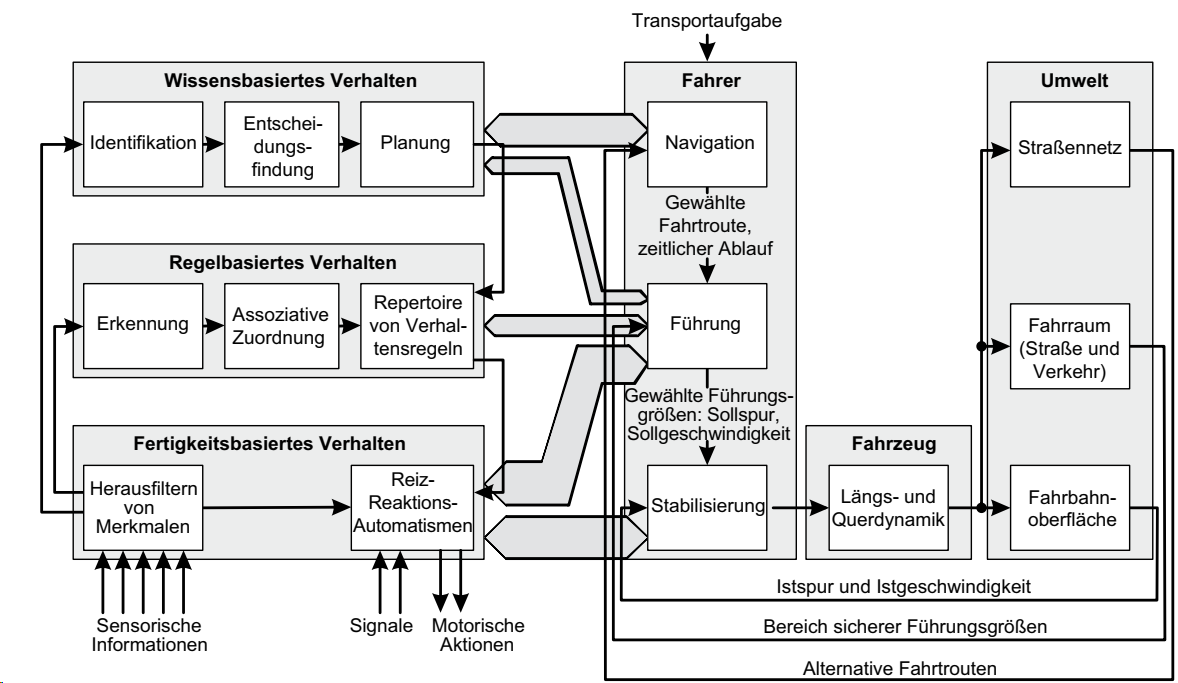
\includegraphics[width=1\textwidth]{images/theory/Modell_Rasmussen.png}
    \caption{Gegenüberstellung von Drei-Ebenen-Modell für zielgerichtete Tätigkeiten des Menschen und Drei-Ebenen-Hierarchie der Fahraufgabe}
    \label{fig:rasmussen}
    \medskip
    {\footnotesize Quelle: Abbildung übernommen aus
    \cite[S.~19]{donges2015fahrerverhaltensmodelle}.}
\end{figure}

Geisler \cite{Geisler_hci2021} unterteilt nach Rasmussen \cite{Rasmussen1983} das menschliche Fahrverhalten in drei Ebenen. Abbildung \ref{fig:rasmussen} zeigt die Gegenüberstellung von Verhaltensweisen des Menschen und Fahraufgaben. Der Forscher konstatiert, dass sich die Verhaltensarten im wesentlichen anhand des Ausmaßes der kognitiven Belastung unterscheiden \cite{Geisler_hci2021}. Während das fertigkeitsbasierte Verhalten unbewusst und als reines Reiz-Reaktions-Schema ablaufe, könne die fahrzeugführende Person beim regelbasierten Verhalten immerhin noch auf sequentiell verknüpfte Schritte zurückgreifen, während das wissensbasierte Verhalten ein bewusstes Überlegen erfordere, so Geisler \cite{Geisler_hci2021}. Desweiteren könnten durch Training und Erfahrung die kognitive Belastung reduziert werden, was zu geringeren Reaktions- und Ausführungszeiten sowie geringerer Ablenkung führe \cite{Geisler_hci2021}. Der Forscher schließt, dass Lernförderlichkeit und Sicherheit des Systems eng miteinander verknüpft seien \cite{Geisler_hci2021}.

Für diese Forschungsarbeit bedeutet dies, dass ein Onboarding für Assistenzsysteme den Anteil an kognitiv fordernden Prozessen möglichst minimieren sollte. Fahrer*innen sollten insbesondere in unübersichtlichen Situationen einzelne Hinweise von Assistenzsystemen schnell zuordnen und wiedererkennen können, ohne, aus Sicht der Fahrzeugsicherheit, lange und damit ungünstige Überlegungen durchführen zu müssen. Außerdem sollte bei Assistenzsystemen, welche möglicherweise seltener zum Einsatz kommen, ein ausführlicheres Onboarding stattfinden, da die Fahrer*innen auf weniger Erfahrungen zurückgreifen können.  

\section{Human Factors im Fahrzeugkontext}
\label{sec:human_factors}
Dieses Unterkapitel betrachtet grundlegende theoretische Modelle und Erkenntnisse, welche in der Literatur \cite{Geisler_hci2021,Geisler_autonom2021} identifiziert wurden und die besonderen Herausforderungen an Gestaltungslösungen im Fahrzeugkontext aufzeigen sollen. Die Erkenntnisse sind einerseits für die Gestaltung einer möglichst realitätsnahen Simulationsumgebung, welche ein Fahrzeug mit seinen Assistenzfunktionen abbildet, relevant. Darüber hinaus werden diese Erkenntnisse für die Gestaltung eines Onbaordings kritisch reflektiert und zueinander in Bezug gesetzt.

\subsection{Wahrnehmung, Aufmerksamkeitssteuerung und mentale Modelle}
\label{subsec:wn_as_mm}

\subsubsection{Visuelle Wahrnehmung}
\label{subsubsec:visuelle_wahrnehmung}
Innerhalb eines Fahrzeugs nutzt der Mensch mehrere Wahrnehmungskanäle, um Informationen wahrzunehmen. Geisler \cite{Geisler_hci2021} nennt neben der visuellen die auditive Wahrnehmung und die taktile Wahrnehmung als wichtigste Informationskanäle.

Bzgl. der visuellen Wahrnehmung sei zentral, dass Menschen trotz eines ca. 180° großen Sichtfeldes nur in einem Bereich von ca. 2° scharf sehen können \cite{Geisler_hci2021}. Außerdem benötige das Scharfstellen der Augen (Akkomodation) sowie die Anpassung der Pupillengrößen an die umgebende Helligkeit (Adaption) Zeit, was mit zunehmenden Alter einer Person an Effektivität verliere, so Geisler \cite{Geisler_hci2021}. Akkomodation sei im Fahrzeugkontext insbesondere dort relevant, wo Blickabwendungen von der Straße aufgrund von Anzeigeelementen im Fahrzeug nötig werden, während Adaption bei großen Helligkeitsunterschieden, welche z. B. durch die Sonne hervorgerufen werden, beachtet werden müssen \cite{Geisler_hci2021}.

Für diese Forschungsarbeit lässt sich ableiten, dass für ein kontextspezifisches Onboarding, welches während der Fahrt stattfindet, insbesondere die Akkomodation eine zentrale Rolle spielt. Es erscheint vor dem Hintergrund der vorgestellten Erkenntnisse sinnvoll, dass Informationen nahe des Blickfelds erscheinen, um langfristige Anpassungsprozesse innerhalb des Auges vermeiden zu können.

\subsubsection{Auditive Wahrnehmung}
\label{subsubsec:auditive_wahrnehmung}
Im Kontext von auditiver Wahrnehmung innerhalb eines Fahrzeugs, sind insbesodnere Warn- und Signaltöne von entscheidender Bedeutung \cite{Geisler_hci2021}. Um eine verlässliche Wahrnehmung von Warn- und Signaltönen gewährleisten zu können, müssen diese hinsichtlich ihrer Beschaffenheit so gewählt werden, dass sie unter Einbezug von verschiedenen Umgebungen sowie Störfaktoren problemlos wahrgenommen werden können \cite{Geisler_hci2021}. Außerdem sollten Klangfarbe, Wiederholfrequenz und Tonhöhe in Abhängigkeit der Dringlichkeit variiert werden und nach Möglichkeit auch eine räumliche Zuordnung des Tons möglich sein \cite{Geisler_hci2021}.

Auch in diesem Fall sind die Erkenntnisse schwerpunktmäßig für ein kontextspezifisches Onboarding während der Fahrt relevant. Trotzdessen, dass eine genaue Lokalisation eines Tons in einer Simulatorumgebung möglicherweise nur mit geeigneten Kopfhörern sinnvoll erscheint, können Klangfarbe, Wiederholfrequenz und Tonhöhe durchaus variiert werden. Dabei sollte für Warnungen

\subsubsection{Taktile Wahrnehmung}
\label{subsubsec:taktile_wahrnehmung}
Die taktile Wahrnehmung habe den zentralen Vorteil, dass es eine große räumliche Nähe zwischen den Extremitäten der fahrzeugführenden Person und dem zu betätigenden Steuerelement gebe, sodass oft keine Zuordnung zwischen Information und Steuerelemtent erfolgen müsse \cite{Geisler_hci2021}. Denkbar seien Vibrationen innerhalb des Sitzes, am Lenkrad oder an einem der Fußpedale des Fahrzeugs \cite{Geisler_hci2021}. 

Aufgrund der Limitationen eines Fahrsimulators, können taktile Informationen nur über die Vibrationen eines Lenkrads bereitgestellt werden. Für die Gestaltung eines Onbaordings erscheint auch dies schwerpunktmäßig für ein kontextspezifisches Onbaording relevant. 

\subsection{Aufmerksamkeitssteuerung}
\label{subsec:aufmerksamkeitssteuerung}

\subsubsection{Informationsverarbeitung}
\label{subsubsec:informationsverarbeitung}
Insbesondere für die visuelle Wahrnehmung, bei der mehrere räumlich verteilte optische Reize, trotz eines nur vergleichsweise kleinen Bereichs des scharfen Sehens miteinander konkurrieren, ist es wichtig zu erörtern, wie die menschliche Aufmerksamkeitssteuerung konzeptionell arbeitet. In der Literatur \cite{Geisler_hci2021} wird zu diesem Zweck oft das SEEV-Modell nach Wickens \cite{Wickens2008} aufgeführt, welches die Wahrscheinlichkeit für die visuelle Wahrnehmung eines Reizes angibt, wenn mehrere miteinander konkurrierende visuelle Reize potentiell ebenfalls wahrgenommen werden könnten. Abbildung \ref{fig:wickens} zeigt den Aufbau des SEEV-Modells nach Wickens \cite{Wickens2008}. Das Modell unterscheidet nach Geisler \cite{Geisler_hci2021} im wesentlichen zwischen Bottom-up, also Aspekten, die durch das Systemdesign direkt beeinflusst werden können und Top-Down, was primär durch Erwartungen und mentale Modelle beeinflusst wird.

\begin{figure}[ht]
    \centering
    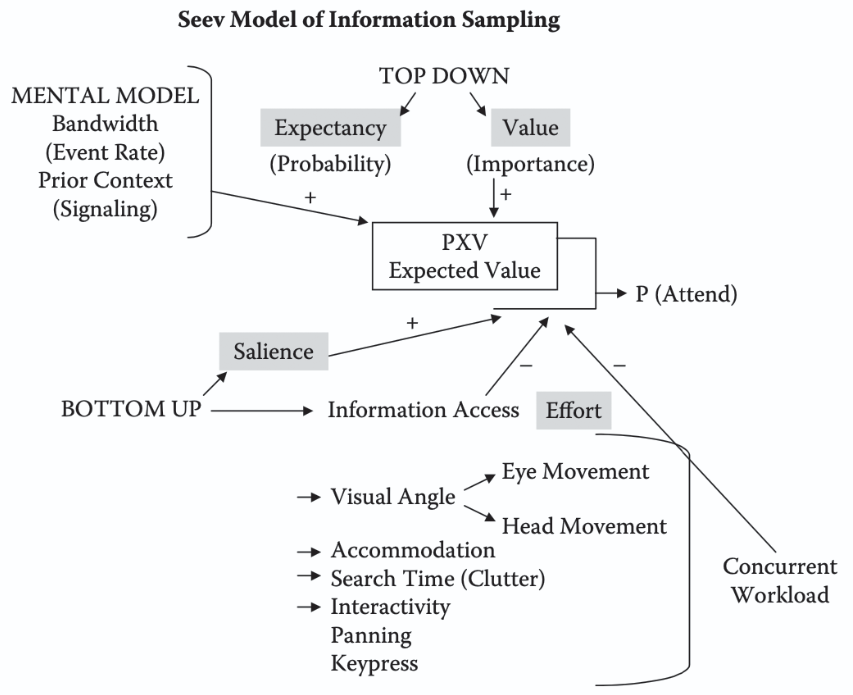
\includegraphics[width=0.8\textwidth]{images/theory/Modell_Wickens.png}
    \caption{SEEV-Modell der Informationsverarbeitung nach Wickens}
    \label{fig:wickens}
    \medskip
    {\footnotesize Quelle: Entnommen aus \cite[S.~23]{Eisma2021} nach \cite{Wickens2008}.}
\end{figure}

Neben den bereits zuvor in Kapitel \ref{subsubsec:visuelle_wahrnehmung} diskutierten Aspekten Auffälligkeit und Anstrengung, sollte für die Entwicklung eines Onbaordings auch die Top-Down-Parameter Erwartbarkeit und Wert beachtet werden. Insbesondere bei kontextspezifischen Onboardings sollten Informationen dort vermittelt werden, wo es die fahrzeugführende Person erwartet. Außerdem sollte der Wert einer sicherheitskritischen Information durch die zuvor diskutierten Gestaltungsmöglichkeiten unterstrichen werden.

\subsubsection{Mentale Modelle}
\label{subsubsec:mentale_modelle}
Die Bedeutung von mentalen Modellen für die visuelle Informationsverarbeitung zeigt Abbildung \ref{fig:wickens}. Allerdings muss an dieser Stelle noch eine Definition und Einordnung von mentalen Modellen erfolgen. Feinauer et al. \cite{feinauer2023first} verstehen mentale Modelle als Wissensstrukturen, die u. a. das Verständnis des Systemumfangs, der Funktionalität und der Gründe für das Systemverhalten umfassen. Norman \cite{Norman1986} beschreibt mentale Modelle als interne Vorstellungen eine*r Nutzer*in darüber, wie ein technisches System aufgebaut ist und funktioniert. Es entsteht auf Grundlage der wahrgenommenen Systeminformationen (System Image) und kann von dem ursprünglichen Designmodell des Entwicklers abweichen \cite{Norman1986}. Abbildung \ref{fig:norman} illustriert die Entstehung eines mentalen Modells. Die Bedeutung von mentalen Modellen, wird im Fahrzeugkontext als wesentlich für eine korrekte und sichere Nutzung eines Fahrzeuges beschrieben \cite{feinauer2022potential}.

\begin{figure}[ht]
    \centering
    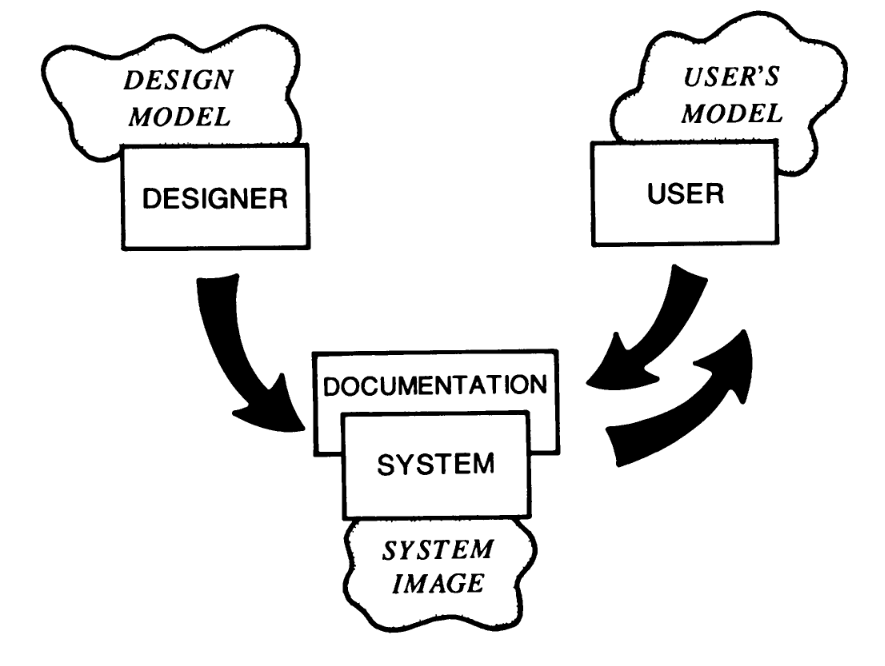
\includegraphics[width=0.5\textwidth]{images/theory/Modell_Norman.png}
    \caption{Zusammenhang zwischen dem Designmodell des Entwicklers, dem Systembild und dem mentalen Modell des Nutzers nach Norman}
    \label{fig:norman}
    \medskip
    {\footnotesize Quelle: Entnommen aus \cite[S.~46]{Norman1986}.}
\end{figure}

\subsection{Situationsbewusstsein}
\label{subsec:situationsbewusstsein}
Geisler \cite{Geisler_hci2021} verweist darauf, dass die im vorherigen Unterkapitel \ref{subsec:wn_as_mm} diskutierten Aspekte nur der erste Teil eines zweistufigen kognitiven Prozesses seien. Der Forscher konstatiert, dass der zweite Teil aus dem Verstehen des Wahrgenommenen, einer Projektion in die Nahe Zukunft und dem Ableiten angemessener Handlungsschritte bestünde \cite{Geisler_hci2021}. Der genauen Ablauf wird in Abbildung \ref{fig:endsley} veranschaulicht. In der Literatur \cite{Geisler_hci2021} wird darauf hingewiesen, dass ein vollständiges Situationsbewusstsein erst nach einem vollständigen Durchlauf aller drei illustrierten Stufen entstehen kann. Als eine mögliche Fehlschlagsursache wird die begrenzte menschliche kognitive Leistungsfähigkeit in Bezug auf Multitasking genannt \cite{Geisler_hci2021}. Die eigentliche Entscheidungsfindung kann schlussendlich automatisiert oder durch Abrufen von zusätzlichen Informationen aus dem Langzeitgedächtnis erfolgen \cite{Geisler_hci2021}. Als eine große Stärke des Modells wird aufgeführt, dass es dazu beitragen könne, den technischen Unterstützungsbedarf für eine fahrzeugführende Person zu ermitteln, da es auch äußere Einflüsse salient mache \cite{Geisler_hci2021}.    

\begin{figure}[ht]
    \centering
    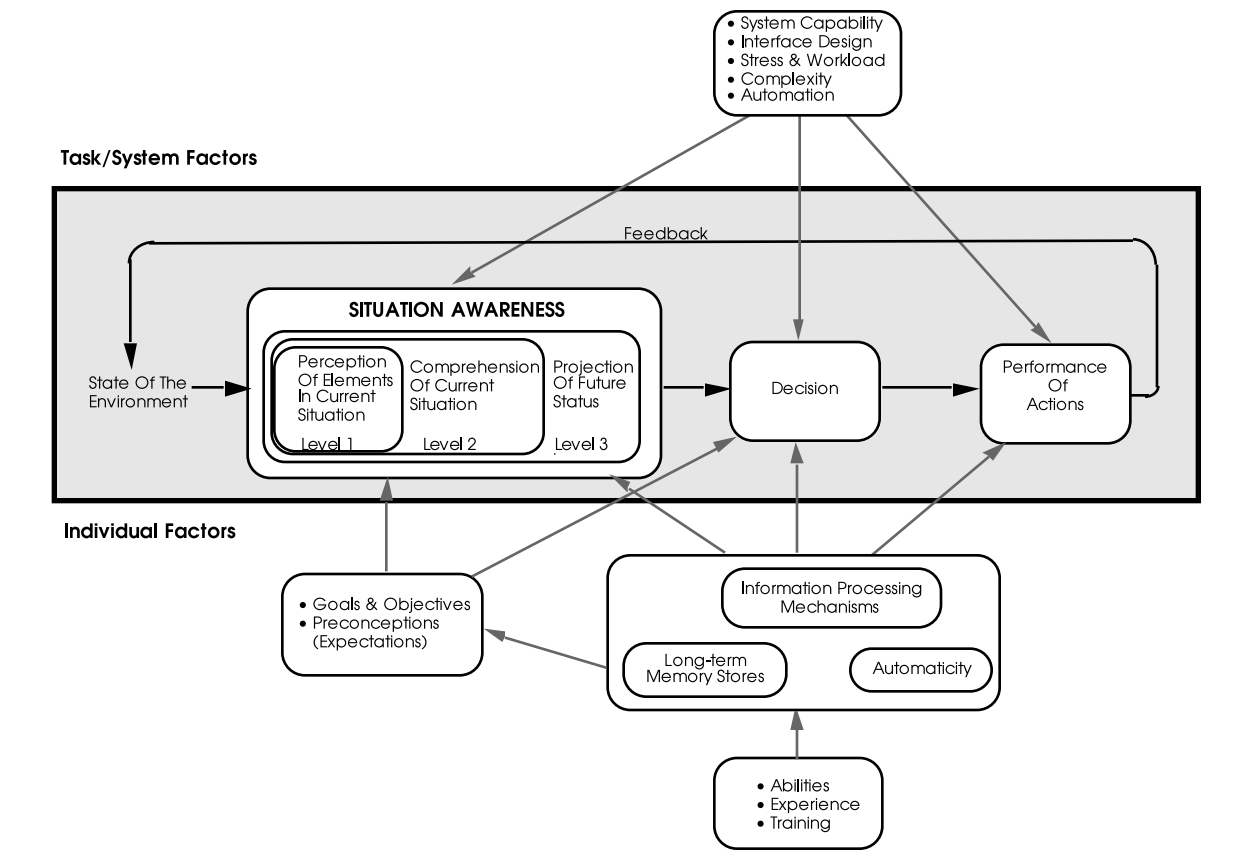
\includegraphics[width=1\textwidth]{images/theory/Modell_Endsley.png}
    \caption{Modell des Situationsbewusstseins in dynamischer Entscheidungsfindung nach Endsley}
    \label{fig:endsley}
    \medskip
    {\footnotesize Quelle: Entnommen aus \cite[S.~3]{Endsley2000Chapter}.}
\end{figure}

Zuletzt wird in der Literatur \cite{Geisler_hci2021} auf die Gefahr von einem negativen Einfluss steigender Automatisierung in Fahrzeugen auf das Situationsbewusstsein der Fahrer*innen hingewiesen, da insbesondere fehlerhafte vollautomatische Handlungen oder Handlungsempfehlungen zu Verwirrungen führen könnten. Die im Kapitel \ref{chapter:introduction} bereits erwähnten Stufen des SAE-Standards \cite{SAE2021J3016} definieren dabei klar, ab welchem Grad der Automatisierung vermehrt Probleme auftreten. Geisler \cite{Geisler_autonom2021} bezeichnet die ersten vier Stufen des SAE-Standards \cite{SAE2021J3016} als Mensch-Maschine-Kooperation, da erst ab den darüberliegenden Stufen eine nahezu vollständige Delegation der Aufgaben einer fahrzeugführenden Person an eine Maschine möglich ist, ohne, dass ein menschliches Eingreifen mittels Übernahmeaufforderung erforderlich wäre. Insbesondere für die Stufen drei und vier, deren zugehörige Fahrzeuge in manchen Situationen die fahrzeugführenden Person zur Übernahme auffordern, müsse ein neues Situationsbewusstsein entstehen, so der Forscher \cite{Geisler_autonom2021}. 

In diesem Zusammenhang wird auch der Begriff 'Mode Awareness' genannt \cite{kurpiers2020mode}. Dieser umfasst das Wissen darüber, welches Automatisierungssystem beziehungsweise welcher Modus momentan aktiv ist, über welches Leistungsvermögen dieser verfügt und welche Aufgaben und Verantwortlichkeiten bei der fahrzeugführenden Person verbleiben \cite{kurpiers2020mode}. Ein angemessenes mentales Modell der Fähigkeiten und Grenzen des Systems ist dabei eine wesentliche Voraussetzung für Mode Awareness \cite{kurpiers2020mode}. Es wird zudem in der Literatur \cite{Geisler_hci2021} diskutiert, dass zusätzliche Erläuterungen des Systems in einer bestimmten Situation zu einer Besserung dieser Problematiken beitragen können. Dies stellt die Notwendigkeit für ein Onbaording, insbesondere eines kontextspezifischen, noch einmal besonders deutlich heraus. Für neue Assistenzfunktionen, deren Verhaltensweisen und Gründe für ein Verhalten weniger bekannt sind, ergäbe  sich möglicherweise mithilfe eines geeigneten Onboardings eine Chance für einen erheblichen Sicherheitsgewinn durch ein besseres Situationsbewusstsein. Zudem sollte ein Onboarding der fahrzeugführenden Person nach einer Übernahmeaufforderung genügend Kontext bieten, um selbstständig Entscheidungen treffen zu können. 

\subsection{Vertrauen, Reliance und Akzeptanz}
\label{subsec:vertrauen_akzeptanz}
Die bisher betrachteten Konzepte zeigen, dass Fahrer*innen sowohl ein angemessenes mentales Modell als auch ein ausreichendes Bewusstsein über den aktuellen Systemzustand benötigen. Diese Kenntnisse bilden zugleich eine Grundlage dafür, die Zuverlässigkeit und Leistungsfähigkeit einer Assistenzfunktion realistisch einzuschätzen. Eine solche Einschätzung ist für die Gestaltung eines Onboardings besonders relevant, da dieses nicht lediglich Wissen vermitteln, sondern auch einer unangemessenen Über- oder Unterschätzung des Systems entgegenwirken sollte. Im Folgenden werden daher Vertrauen, Reliance und Akzeptanz als weitere Einflussgrößen der Nutzung von Fahrassistenzsystemen betrachtet.

\subsubsection{Vertrauen und Reliance}
An dieser Stelle sollen zunächst Vertrauen und Reliance klar voneinander abgegrenzt werden. Körber et al. \cite{korber2018introduction} verstehen Vertrauen als Einstellung gegenüber dem automatisierten System, während Reliance als beobachtbares 'Sich-Verlassen' auf das System verstanden wird. Insgesamt sei es wichtig, dass ein angemessenes und kalibriertes Vertrauen angestrebt werde, so die Forscher*innen \cite{korber2018introduction}. Dies begründen Körber et al. \cite{korber2018introduction} mit den Ergebnissen aus einer von ihnen durchgeführten Studie mit einem Fahrzeug innerhalb eines Fahrsimulators, welches Stufe drei des SAE-Standards zugeordnet werden kann \cite{SAE2021J3016}. Vertrauensfördernde Informationen führten zu stärkerer Reliance, geringerer Überwachung und schlechterem Übernahmeverhalten, was bei vereinzelten Studienteilnehmer*innen sogar zu Kollisionen führte.

\begin{figure}[ht]
    \centering
    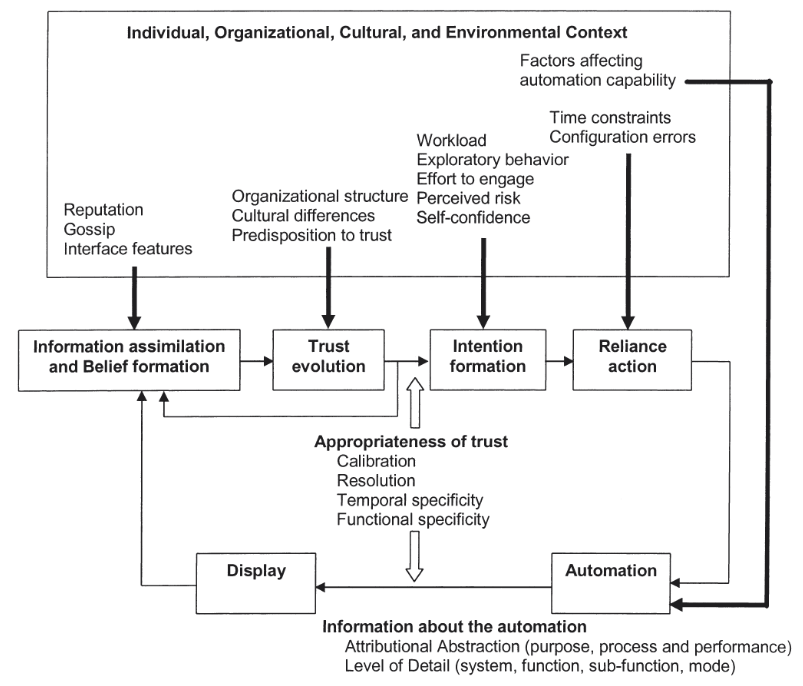
\includegraphics[width=0.8\textwidth]{images/theory/Modell_TIA.png}
    \caption{Trust In Automation Modell nach Lee \& See}
    \label{fig:tia}
    \medskip
    {\footnotesize Quelle: Entnommen aus \cite[S.~19]{lee2004trust}.}
\end{figure}

Vertrauen und Reliance können auch anhand eines konzeptionellen Modells von Lee \& See \cite{lee2004trust} voneinander abgegrenzt werden. Lee \& See \cite{lee2004trust} definieren Vertrauen in Automation als die Einstellung, dass ein automatisiertes System eine Person bei der Erreichung ihrer Ziele in einer Situation unterstützt, die durch Unsicherheit und
Verletzlichkeit gekennzeichnet sei. Vertrauen sei damit zunächst
von dem tatsächlich beobachtbaren Nutzungsverhalten abzugrenzen \cite{lee2004trust}. Während Vertrauen eine innere Bewertung der Automation beschreibe, bezeichne Reliance das konkrete Verhalten, sich bei der Erfüllung
einer Aufgabe auf das System zu verlassen \cite{lee2004trust}. Zur Beschreibung der Grundlagen von Vertrauen unterscheiden Lee \& See \cite{lee2004trust} zwischen den Ebenen Performance, Process und
Purpose. Performance umfasse das beobachtbare Leistungsvermögen und
die Zuverlässigkeit eines Systems \cite{lee2004trust}. Process beziehe sich auf die Funktionsweise und die Nachvollziehbarkeit der Prozesse, durch die
das System zu seinem Verhalten gelangt \cite{lee2004trust}. Purpose beschreibe den vorgesehenen Zweck, die Ziele und den Nutzungskontext der Automation \cite{lee2004trust}. Die drei Ebenen  würden es Nutzer*innen ermöglichen, die Vertrauenswürdigkeit eines Systems sowohl anhand seines beobachtbaren Verhaltens als auch anhand seiner Funktionsweise und seines vorgesehenen Einsatzbereichs einzuschätzen, so die Forscher*innen \cite{lee2004trust}. Abbildung \ref{fig:tia} zeigt das Modell.

Beggiato \& Krems \cite{beggiato2013evolution} konnten zudem zeigen, dass vorab bekannte Systemgrenzen sich nicht zwangsläufig negativ auf Vertrauen und Akzeptanz auswirken. Kraus et al. \cite{kraus2020more} greifen zudem die im Kapitel \ref{subsec:situationsbewusstsein} diskutierten negativen Einflüsse von Systemfehlern auf. Werden mögliche Systemgrenzen transparent kommuniziert, könne ein starker Vertrauensabfall nach dem Auftreten eines Systemfehlers abgemildert oder verhindert werden, so die Forscher*innen.

Für die Gestaltung eines Onboardings folgt daraus, dass nicht lediglich die Bedienung einer Assistenzfunktion vermittelt werden sollte. Nutzer*innen benötigen ebenfalls Informationen darüber, welche Leistungen das System erbringen kann, unter welchen Bedingungen und auf welcher Grundlage es arbeitet und für welche Situationen es vorgesehen ist. Ein Onboarding sollte daher die Leistungsfähigkeit und Grenzen der Assistenzfunktion, ihre grundlegende Funktionsweise und relevanten Systemzustände sowie ihren Zweck und die verbleibende Verantwortung der fahrzeugführenden Person vermitteln. Ziel ist dabei nicht die Maximierung des Vertrauens. Vielmehr sollte das Onboarding eine realistische Einschätzung der Systemfähigkeiten fördern, sodass das Vertrauen und das tatsächliche Sich-Verlassen auf die Assistenzfunktion möglichst mit deren objektiver
Leistungsfähigkeit übereinstimmen.

\subsubsection{Akzeptanz}
Auch das Konstrukt der Akzeptanz, soll anhand eines theoretischen Modells in den Fahzeugkontext eingeordnet werden. Osswald et al. \cite{osswald2012predicting} kritisieren, dass etablierte Modelle, bspw. das Technologie-Akzeptanz-Modell \cite{davis1989technologyacceptance}, zur Untersuchung von Technologien in Fahrzeugen unzureichend seien, da diese ursprünglich für stationäre Computersysteme und organisationale Nutzungskontexte etwickelt worden wären. Außerdem würden Besonderheiten des Fahrens, bspw. die Bewegung des Fahrzeugs, wechselde Umweltbedingungen, begrenzte kognitive Ressourcen und das mit der Nutzung verbundene Sicherheitsrisiko nur unzureichend berücksichtigt, so die Forscher*innen \cite{osswald2012predicting}. Detjen et al. \cite{detjen2021increase} stützen diese Erkenntnisse im Hinblick darauf, dass Akzeptanz von mehreren Faktoren wie wahrgenommener Sicherheit, Kontrolle, Nützlichkeit und postiver Nutzungserfahrung abhänge. Das Car Technology Acceptance Model (CTAM) nach Osswald et al. \cite{osswald2012predicting} stellt eine auf fahrzeuginterne Informationstechnologien zugeschnittene Erweiterung der Unified Theory of Acceptance and Use of Technology (UTAUT) \cite{venkatesh2003utaut} dar. Neben den aus der UTAUT übernommenen Konstrukten Performance Expectancy, Effort Expectancy, Social Influence und Facilitating Conditions umfasst das CTAM daher auch Attitude Towards Using Technology, Self-Efficacy, Anxiety und Perceived Safety. Diese Faktoren sollen die Nutzungsabsicht beziehungsweise das tatsächliche Nutzungsverhalten beeinflussen. Abbildung \ref{fig:ctam} zeigt das CTAM.

\begin{figure}[ht]
    \centering
    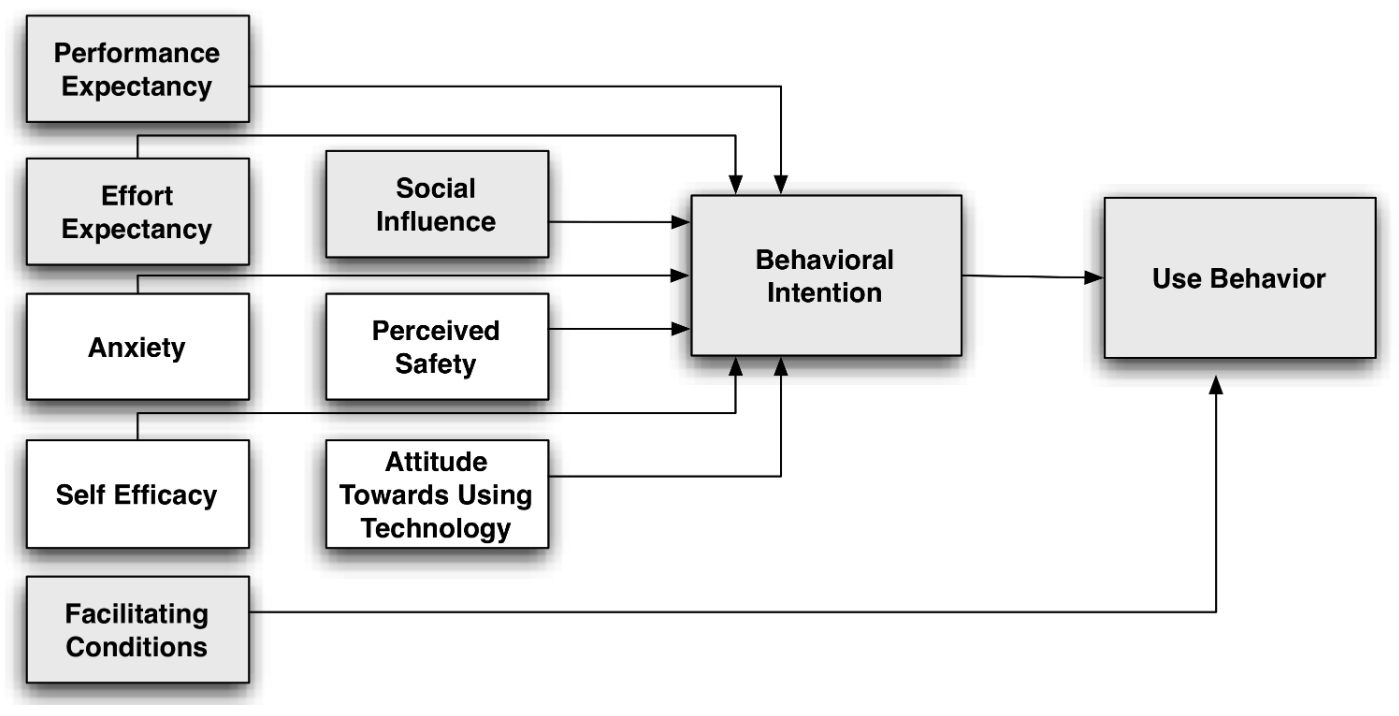
\includegraphics[width=0.8\textwidth]{images/theory/Modell_CTAM.png}
    \caption{Car Technology Acceptance Research Model nach Osswald et al.}
    \label{fig:ctam}
    \medskip
    {\footnotesize Quelle: Entnommen aus \cite[S.~5]{osswald2012predicting}.}
\end{figure}

Für die vorliegende Arbeit sind insbesondere Effort Expectancy,
Facilitating Conditions, Self-Efficacy, Anxiety und Perceived Safety
relevant. Ein Onboarding sollte die wahrgenommene Verständlichkeit und
Erlernbarkeit einer Assistenzfunktion unterstützen, als integriertes
Hilfs- und Lernangebot dienen, die wahrgenommene eigene Kompetenz
fördern und Unsicherheiten hinsichtlich der sicheren Nutzung reduzieren.

Das später entwickelte Autonomous Vehicle Acceptance Model (AVAM)
nach Hewitt et al. \cite{hewitt2019assessing} greift die Konstrukte
des CTAM \cite{osswald2012predicting} auf und überträgt sie auf die Akzeptanz automatisierter Fahrzeuge unterschiedlicher Automatisierungsstufen. Da in der
vorliegenden Arbeit jedoch nicht die Akzeptanz eines automatisierten
Fahrzeugs als Gesamtsystem, sondern die Nutzung ausgewählter
Fahrassistenzfunktionen betrachtet wird, stellt das CTAM den
passenderen theoretischen Bezugsrahmen dar.

\section{Defizite der gegenwärtigen Informationsvermittlung in Bezug auf ADAS}
\label{sec:informationsdefizite}

Nachdem in den Kapiteln \ref{sec:fas_sicherheitskritisch} und \ref{sec:human_factors} die Rolle der fahrzeugführenden Person sowie grundlegende Modelle und Erkenntnisse für Gestaltungslösungen im Fahrzeugkontext diskutiert wurden, werden in diesem Unterkapitel Defizite bei der Informationsvermittlung in Bezug auf Fahrassistenzsysteme aufgezeigt. Im Folgenden wird die Begriffichkeit Advanced Driving Assistance Systems (ADAS) für Systeme verwendet, die Fahrer*innen bei der Fahraufgabe unterstützen. Die Unterstützung kann durch die Bereitstellung von Informationen und
Warnungen sowie durch zeitweise oder dauerhafte Eingriffe in die
Längs- und/oder Querführung des Fahrzeugs erfolgen. ADAS ersetzen
die fahrzeugführende Person jedoch nicht. Die Verantwortung für die
Fahrzeugsteuerung und die Überwachung der Umgebung sowie der
Systemleistung verbleibt bei ihr \cite{UNECE2024ADAS}.

\subsection{Fehlvorstellungen und nicht intendierte Nutzung}
\label{subsec:fehlvorstellungen_fehlgebrauch}
Ayoub et al. \cite{ayoub2022cause} führten ein Literaturreview zu ADAS-Limitationen und Lösungen durch und analysierten Verbraucherbeschwerden aus einer Datenbank. Laut den Forscher*innen \cite{ayoub2022cause} seien Problematiken in Bezug auf ADAS oft mit menschlichem Fehlverhalten assoziiert, wozu missbräuchliche Nutzung, Nicht-Nutzung, falsches Vertrauen, Übervertrauen und Missverständnisse über Systemfähigkeiten und Systemgrenzen zählen würden. Die Forschungsarbeit \cite{ayoub2022cause} beschreibt mit Regen, Schnee, Nebel, Eis, Gegenlicht, Dunkelheit, verdeckten oder unklaren Fahrbahnmarkierungen, schlechten Straßenbedignungen oder verdeckten Sensoren auch eine Reihe von Umweltgrenzen, welche die Systemleistung negativ beeinträchtigen können. Die Verbraucherbeschwerden sähen die zentrale Ursache jedoch nicht im eigenem Fehlverhalten, welches die Grenzen der Systeme missachte, sondern in generellen Fahrzeug- und Systemproblemen, so die Forscher*innen \cite{ayoub2022cause}. Besonders häufig genannt wurden unbekannte Ursachen, Fehlalarme, Nicht-Reagieren des Systems, Rückrufe sowie Sensor- und Software-Probleme \cite{ayoub2022cause}. Auch die an die Problematiken anschließenden Folgen wurden untersucht. Demnach seien ein ADAS-Ausfall, starkes Bremsen, Warnmeldungen, Kollisionen und Beinahe-Kollisionen jene Aspekte, welche am häufigsten genannt wurden \cite{ayoub2022cause}. Außerdem konnten ADAS-spezifische Unterschiede zwischen den Systemen beobachtet werden, sodass bspw. bei einem Notbremsungs-System häufiger Fehlalarme aufträten, während bei einem Spurhalteassistent vermehrt Probleme bzgl. eines Nicht-Reagierens zu beobachten seien \cite{ayoub2022cause}. 

Für das Design eines Onboardings für Assistenzsysteme lässt sich ableiten, dass Systemgrenzen klar und transparent kommuniziert werden müssen. Darüber hinaus sollten Onboardings möglichst funktionsspezifisch gestaltet sein, sodass eine oberflächliche Erklärung nicht zielführend erscheint.

Novakazi et al. \cite{novakazi2025mind} stützen diese Erkenntnisse. Zu diesem Zweck führten Novazaki et al. \cite{novakazi2025mind} eine Studie durch, in der 16 Teilnehmer*innen auf öffentlichen Straßen in einem modifizierten Volvo X90 mit zwei unterschiedlichen Interfaces fuhren. Während das erste Interface Informationen zu automatisierten Fahrfunktionen auf das nötigste reduzierte, wurde das zweite expliziter gestaltet, mit klaren visuellen Hinweisen zu Systemstatus, Verantwortung und Automationsmodus \cite{novakazi2025mind}. Es zeigte sich, dass auch jene Teilnehmer*innen, welche über das informationstechnisch reichhaltigere Interface verfügten, auffällig viele Fehler machten \cite{novakazi2025mind}. Die Autor*innen \cite{novakazi2025mind} argumentieren, dass Missbrauch und Fehlbedienung von automatisierten Fahrfunktionen demnach nicht allein durch UI-Probleme erklärbar seien. Stattdessen würden vorherige Erwartungen, Medienbilder, Erfahrungen mit anderen Assistenzsystemen und falsche Vorstellungen über Systemfähigkeiten eine zentrale Rolle spielen, so die Forscher*innen \cite{novakazi2025mind}. 

Diese Erkenntnisse sind für die Entwicklung eines eigenen Onbaordings zentral, da sie darauf hindeuten, dass ein Onbaording nicht isoliert von Ereignissen aus der Vergangenheit betrachtet werden kann. Vielmehr müssen vorbestehende Erwartungen teilweise aktiv korrigiert werden. Außerdem sollten die Unterschiede zwischen Assistenz und Automation noch einmal besonders betont werden, um die Sicherheit zu erhöhen.

Auch der Einfluss der im Kaptitel \ref{subsec:aufmerksamkeitssteuerung} beschriebenen mentalen Modelle, spielt in diesem Zusammenhang eine große Rolle. Gaspar et al. \cite{gaspar2020impact} untersuchten in einer Studie, wie die Qualität des mentalen Modells von Fahrerinnen und Fahrern zu Adaptive Cruise Control (ACC) ihre Leistung in kritischen Grenzsituationen beeinflusst. Die Gruppe der Fahrer*innen war divers hinsichtlich der Fahrerfahrung und des Alters, und unterschied sich demnach im Umfang und Qualität des mentalen Modells zu dieser Assistenzfunktion \cite{gaspar2020impact}. Insbesondere das Verständnis über die Grenzen des Systems, war in der Gruppe mit einem schwachen mentalen Modell deutlich weniger stark ausgeprägt, als bei Vorhandensein eines starken mentalen Modells \cite{gaspar2020impact}. Ein starkes mentales Modell, führte zudem zu einem schnelleren Eingreifen, wenn ACC nicht reagierte, während Personen mit einem schwachen mentalen Modell Hindernissen deutlich näher kamen \cite{gaspar2020impact}.

Da die Güte des mentalen Modells mit einfachen Fragen zur Assistenzfunktion überprüfbar war \cite{gaspar2020impact}, könnte dies auch für ein Onboarding umgesetzt werden, sodass Onboardings mit einer unterschiedlichen Informationstiefe angeboten werden könnten. Allerdings ist die wesentliche Erkenntnis in diesem Fall, dass mentale Modelle als sicherheitsrelevant angesehen werden müssen.

\subsection{Fahrzeughandbücher, Demografie, Fahrzeugkauf und Fahrausbildung}
\label{subsec:informationsquellen}
abc

\subsection{Kommunikation von Systemfähigkeiten und Systemgrenzen}
\label{subsec:kommunikation_systemgrenzen}
abc


\section{Training und Onboarding für Fahrassistenzsysteme}
\label{sec:training_onboarding}

\subsection{Begriffsverständnis und Ziele des Onboardings}
\label{subsec:onboarding_begriff}
abc

\subsection{Lerninhalte eines Onboardings}
\label{subsec:onboarding_lerninhalte}
abc

\subsection{Zeitpunkt und Nutzungskontext der Informationsvermittlung}
\label{subsec:onboarding_zeitpunkt}
abc

\subsection{Vermittlungsformen und Interaktionskonzepte}
\label{subsec:onboarding_vermittlungsformen}
abc

\subsection{Motivation, Personalisierung und adaptive Unterstützung}
\label{subsec:onboarding_adaptivitaet}
abc

\subsection{Empirische Befunde zur Wirksamkeit}
\label{subsec:onboarding_wirksamkeit}
abc


\section{Partizipative Entwicklung von In-Car-Onboardings}
\label{sec:partizipative_entwicklung}

\subsection{Grundlagen des partizipativen Designs}
\label{subsec:grundlagen_partizipatives_design}
abc

\subsection{Nutzer*innen als Expert*innen ihrer Nutzungserfahrungen}
\label{subsec:nutzende_expertinnen}
abc

\subsection{Überführung von Nutzer*innenbedarfen in Gestaltungsanforderungen}
\label{subsec:anforderungsableitung}
abc


\section{Evaluation von Onboardings für Fahrassistenzsysteme}
\label{sec:evaluation_onboarding}

\subsection{Evaluationskriterien und Zielgrößen}
\label{subsec:evaluationskriterien}
abc

\subsection{Erfassung mentaler Modelle und Systemverständnis}
\label{subsec:messung_mentale_modelle}
abc

\subsection{Verhaltens- und leistungsbezogene Evaluation}
\label{subsec:verhaltensmessung}
abc

\subsection{Fahrsimulatoren als Evaluationsumgebung}
\label{subsec:fahrsimulator}
abc


\section{Synthese des Forschungsstands und Forschungslücke}
\label{sec:synthese_forschungsluecke}